\section{Робота з даними}
\label{sec:data}

У контексті планування та оптимізації маршрутів ефективна обробка даних відіграє вирішальну роль у перетворенні необроблених даних з баз даних у графічне представлення, яке можна використовувати для розрахунків маршрутів. Цей підрозділ присвячений аспектам обробки даних, пов'язаним зі створенням моделей даних і перетворенням інформації з бази даних у графічну структуру.

Першим кроком в обробці даних є розуміння вимог до даних для планування маршруту. Це передбачає визначення необхідних атрибутів і сутностей, що стосуються транспортної мережі, таких як зупинки, маршрути, розклади, відстані та інша пов'язана з ними інформація. Після визначення вимог до даних можна розробити відповідну модель даних для ефективної організації та представлення цієї інформації.

Як правило, для зберігання даних, пов'язаних з транспортом, використовуються реляційні бази даних, що дозволяють структурувати їх та ефективно здійснювати запити. Дані організовані в таблиці, кожна з яких представляє певний об'єкт або аспект транспортної мережі. Наприклад, можуть бути таблиці для зупинок, маршрутів, розкладів і відстаней, з відповідними зв'язками, встановленими між ними.

Для того, щоб перетворити інформацію з бази даних у графічне представлення, виконується вилучення та перетворення даних. Це передбачає вилучення відповідних даних з таблиць бази даних та їх структурування таким чином, щоб їх можна було представити у вигляді вузлів та ребер графа. Кожна зупинка стає вузлом графа, а зв'язки між зупинками, такі як маршрути або відстані, зображуються ребрами.

На етапі обробки даних можна використовувати різні методи та інструменти для забезпечення ефективного і точного перетворення даних. Це може включати очищення, перевірку та попередню обробку даних для усунення невідповідностей, відсутніх значень або проблем з якістю даних. Крім того, можуть бути застосовані методи інтеграції даних для консолідації даних з різних джерел, що дасть змогу отримати комплексне уявлення про транспортну мережу.

Після того, як дані оброблені і перетворені в графічне представлення, стає легше застосовувати графові алгоритми і виконувати розрахунки маршрутів. Графова структура дозволяє застосовувати алгоритми ефективного обходу, пошуку шляхів та оптимізації для визначення найкоротших маршрутів з урахуванням різних обмежень, таких як відстань, час або інформація про розклад.

Отже, обробка даних є важливим компонентом проектів планування маршрутів. Розробляючи відповідні моделі даних, вилучаючи необхідну інформацію з баз даних і перетворюючи її в графічне представлення, проект може використовувати можливості графових алгоритмів для розрахунку оптимізованих маршрутів. Ефективна обробка даних забезпечує отримання точних, актуальних і структурованих даних, які є основою для ефективного планування та оптимізації маршрутів у транспортних системах.

\subsection{Проектування моделей даних}
\label{subsec:data-models}

Добре розроблена модель даних є основою для точного представлення і маніпулювання транспортною мережею та пов'язаними з нею об'єктами. Основна мета моделі даних - зафіксувати основні елементи, такі як зупинки, маршрути, розклади та їх взаємозв'язки, забезпечуючи комплексне представлення транспортної системи. Це дозволяє ефективно зберігати, знаходити та маніпулювати даними, що дає нам змогу виконувати різні аналізи та операції з пошуку маршрутів.

Під час процесу моделювання даних ретельна увага приділяється відповідним структурам даних і взаємозв'язкам для точного відображення реальної транспортної мережі. Це передбачає визначення таких об'єктів, як вузли (що представляють зупинки або місця), ребра (що представляють сполучення між зупинками) та атрибути, які описують різні властивості цих об'єктів.

Для представлення моделі даних ми використовуємо поєднання концепцій реляційних баз даних та графових структур даних. Реляційні бази даних забезпечують структурований підхід для зберігання та запитів до великих обсягів даних, в той час як графи пропонують інтуїтивно зрозуміле представлення зв'язків між об'єктами, що робить їх ідеальними для сценаріїв планування маршрутів.

Використовуючи можливості моделі даних, пристосованої до конкретних потреб, можна ефективно вирішувати завдання зберігання, пошуку та маніпулювання даними. Це закладає основу для наступних етапів проекту, включаючи реалізацію алгоритмів та оптимізацію маршрутів.

Модель "Station" слугує фундаментальною сутністю для представлення окремих зупинок або місць у транспортній мережі. Вона містить основну інформацію, таку як назва або ідентифікатор станції, географічні координати, що визначають її точне місцезнаходження,  створюючи чітку структуру категоризації.

Модель "Route" відіграє центральну роль у визначенні конкретних маршрутів або ліній у транспортній системі. Вона інкапсулює такі важливі атрибути, як назва або ідентифікатор маршруту. Крім того, модель "Route" встановлює зв'язок "багато-до-багатьох" з моделлю "Station", що дозволяє нам точно представити послідовність зупинок на маршруті.

Для відображення з'єднань або зв'язків між "Station" та "Route" ми використовуємо модель "Connection". Ця модель включає такі поля, як станція відправлення та станція призначення, що представляють початкову та кінцеву точки з'єднання відповідно. Вона також включає такі атрибути, як розклад відправлень.

Для відображення проміжків, з яких складається "Connection" розроблена модель "Waypoint". Вона представляє відрізок між зупинками(на станціях представлених моделлю "Station"). Ця модель дозволяє відображати проміжні точки або зупинки на маршруті, що сприяє точному моделюванню та ефективній обробці даних. Підтримуючи зв'язок з моделями "Station" та "Route", модель "Waypoint" фіксує пов'язану станцію для кожної точки маршруту і забезпечує збереження порядку або послідовності точок на маршруті.

\begin{figure}[!h]
    \centering
    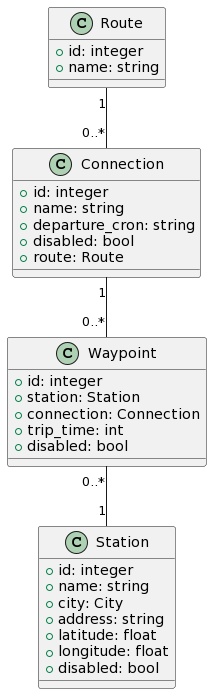
\includegraphics[scale=0.6]{content/chapters/2-implementation-methods/assets/img/models_diagram.png}
    \caption{Діаграма описаних моделей}
    \label{fig:bfs}
\end{figure}


Включаючи ці ретельно розроблені моделі в наш проект, ми створюємо надійну і структуровану структуру представлення даних. Ця основа дозволяє нам ефективно працювати з різноманітними типами транспорту та конфігураціями маршрутів. Модель Station забезпечує детальне представлення окремих зупинок, модель Route відображає загальну структуру маршрутів, модель Connection встановлює зв'язки між станціями, а модель Waypoint враховує складні конфігурації маршрутів. Разом ці моделі забезпечують ефективне зберігання, пошук та маніпулювання даними транспортної системи, сприяючи точному та оптимізованому плануванню маршрутів.

\subsection{Алгоритм перетворення даних в граф}
\label{subsec:models-to-graph}

Щоб забезпечити ефективне планування маршрутів і навігацію в транспортній системі, моделі даних, що представляють станції, маршрути, пересадки і пункти призначення, повинні бути перетворені в графову структуру. Таке графове представлення дозволяє застосовувати різні графові алгоритми, такі як алгоритм Дейкстри або алгоритм Єна, для пошуку найкоротших маршрутів і оптимізації навігації.

Перетворення починається з того, що кожна станція(представлена моделлю "Station") розглядається як вершина графа. Унікальні ідентифікатори станцій, такі як їхні ідентифікатори, можуть бути використані як ідентифікатори для відповідних вузлів.

З'єднання між станціями представлені моделлю "Waypoint", відображаються у вигляді ребер на графі. Кожне ребро представляє прямий зв'язок між двома станціями, використовуючи час подорожі між ними як вагу ребра. Атрибути з'єднання, такі як ідентифікатор станції відправлення, ідентифікатор станції призначення, час подорожі, розклад відправлення, пов'язані з відповідним ребром, потрібно зберігати, щоб використовувати ці дані в подальшій обробці.

Крім того, маршрутні точки, пов'язані з кожним маршрутом, слугують проміжними пунктами на маршруті. Ці точки можуть бути представлені у вигляді вузлів на графі і з'єднані з відповідними станціями ребрами. Таке включення маршрутних точок підвищує точність і гнучкість планування маршруту, дозволяючи здійснювати більш точну навігацію.

Після перетворення моделей у графове представлення можна застосовувати широкий спектр графових алгоритмів для пошуку найкоротших маршрутів, врахування розкладів та оптимізації навігації на основі певних критеріїв. Графова структура забезпечує потужну та гнучку основу для планування маршрутів у транспортній системі, забезпечуючи ефективну та надійну навігацію для користувачів.

\begin{figure}[!h]
    \centering
    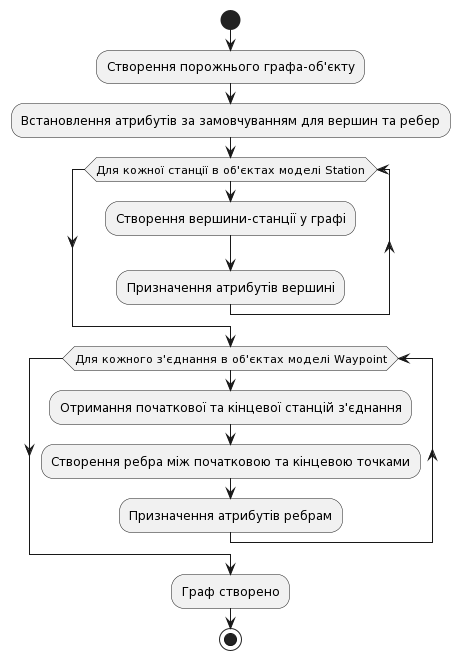
\includegraphics[scale=0.6]{content/chapters/2-implementation-methods/assets/img/models-to-graph_diagram.png}
    \caption{Діаграма описаних моделей}
    \label{fig:bfs}
\end{figure}